\documentclass[]{tudelft-AE-report}

%% Set up the bibliography with natbib
\usepackage[numbers,sort&compress]{natbib}
\bibliographystyle{tudelft-AE-report}  % Use your provided .bst file

%% Other packages
\usepackage{tabularray}
\usepackage{csquotes}
\usepackage{hyperref}
\usepackage{varioref}
\usepackage{cleveref}
\usepackage{todonotes}
\usepackage{amsmath}
\usepackage{amssymb}
\usepackage{calc}
\usepackage{gensymb}
\usepackage{siunitx}
\usepackage{adjustbox} 
\usepackage[table]{xcolor} % Required for coloring table cells
\usepackage{array}         % Required for centering text in tables
\usepackage[labelfont={bf}, 
            textfont={it}, 
            tableposition=top,
            justification=centering]{caption}
\usepackage{float}
\usepackage{graphicx}
\usepackage{wrapfig}
\usepackage{subcaption}
\usepackage{tikz}
\usepackage{array}
\usepackage{booktabs}
\usepackage{longtable}
\usepackage{multicol}
\usepackage{multirow}
\usepackage{enumitem}
\usepackage{easylist}
\usepackage{listings}
\usepackage{color}
\usepackage{changes}
\usepackage{comment}
\usepackage{fancyvrb}
\usepackage{lipsum}
\usepackage{textcomp}
\usepackage{url}
\usepackage{verbatim}
\usepackage{geometry}
\usepackage{nomencl}
\usepackage{pdfpages}
\usepackage{pgfgantt} % required for a gantt chart
\usepackage{lscape} % To make something in landscape
\usepackage{multicol}
\usepackage{tabularx}
\usepackage{diagbox}
\usepackage{pdflscape}
\usepackage{rotating}
\def\AR{\clipbox{0pt 0pt .32em 0pt}\AE\kern-.30emR}


% The following add capital letters to all autoref command outputs
\addto\extrasenglish{%
    \def\chapterautorefname{Chapter}%
    \def\sectionautorefname{Section}%
    \def\subsectionautorefname{Section}%
    \def\subsubsectionautorefname{Section}%
    \def\paragraphautorefname{Paragraph}%
    \def\subparagraphautorefname{Subparagraph}%
    \def\equationautorefname{Equation}
    \def\tableautorefname{Table}
    \def\figureautorefname{Figure}
    \def\footnoteautorefname{Footnote}
    \def\Listautorefname{List}
}

\begin{document}
%% ################### FRONT MATTER ###################
%% Use Roman numerals for the page numbers of the title pages and table of contents.
%\frontmatter
%% The following lines can be used to configure options for the front cover
\titleoffsetx{2cm}
\titleoffsety{14cm+11pt}
\afiloffsetx{49pt}
\afiloffsety{24.2cm} 


\frontboxwidth{17cm-11pt}
\frontboxheight{12cm}
\splitboxheight{12.5cm}

\title{
    \fontsize{50}{40}\selectfont
    {Prelim. Wing Structural Design}}
\subtitle{Work Package 4, Design Report}

\affiliation{Delft University of Technology}
%\covertext{}
\coverimage{cover/B747 Component Diagram.jpg}

%% Uncomment the next line if you want to use only a single author.
%\author{J.\ Random Author}


%% Uncomment the next 21 lines if you want to use multiple authors.
\author{\Large{Group B06,} \Large{ \space AE2111-I System Design } \Large{\space}\\ [1em]
%\todo{Any way to make the fonts the same size?}}\\[1em]
 \newline 
 \large{
 \begin{tabular}{@{}llp{0mm}ll@{}}
     González Piñeiro, Mario & 5761549 && Koot, Sandor & 5998964 \\ Koppejan, Jeroen & 5785928 && Kort, Caelan & 5996740 \\ Lammers, Sander & 5948339 && Putin Frances, Giulia & 5910412 \\ Skrobanek, Hanna & 5908663 && van Steenberge, Nathan & 5957206 \\ Strózik, Mikołaj & 5935776 && Tabără, Andrei-Cristian & 5985161 \\ Talan, Tin & 5973562 && & 
 \end{tabular}
 }}

\makecover[fillboxes]                   % The 'back' option enables the generation of the back cover.
\pagenumbering{Roman}   % Start with Roman numerals
\setcounter{page}{1}    % Ensure page numbering starts at i

%% The following lines force creates an empty page before the titlepage
\thispagestyle{empty}
\vspace{2cm}
\begin{center}
    This page is intentionally left blank.
\end{center}
\newpage


%% The following lines actually make the title page
\begin{titlepage}


\begin{center}

%% Insert the TU Delft logo at the bottom of the page.

%% Print the title in cyan.
{\makeatletter
\largetitlestyle\fontsize{26}{26}\selectfont\@title
%\largetitlestyle\color{tudelft-cyan}\Huge\@title
\makeatother}

%% Print the optional subtitle in black.
{\makeatletter
\ifx\@subtitle\undefined\else
    \bigskip
   {\tudsffamily\fontsize{22}{32}\selectfont\@subtitle}    
    %\titlefont\titleshape\LARGE\@subtitle
\fi
\makeatother}

\bigskip
\bigskip

by
%door

\bigskip
\bigskip

%% Print the name of the author.
{\makeatletter
%\largetitlefont\Large\bfseries\@author
\largetitlestyle\fontsize{26}{26}\selectfont\@author \makeatother}

\bigskip
\bigskip


\vfill

\begin{tabular}{lll}
  
    Project duration: & \multicolumn{2}{l}{Sep, 2024 -- Jan, 2025} \\
    Project supervisor: & M. Pluciński , TU Delft Teaching Assistant \\
    Cover image:   & Marsden, J. A., \textit{Flight International Magazine} (1968) \cite{Marsden1968Flight94}\\
\end{tabular} 
%% Only include the following lines if confidentiality is applicable.

\bigskip
\bigskip
Delft, December 2024

\bigskip
\bigskip
\emph{This report is confidential and cannot be made public.}



%\centering{
\includegraphics{cover/logo_black}}


\end{center}

\begin{tikzpicture}[remember picture, overlay]
    \node at (current page.south)[anchor=south,inner sep=0pt]{
        
\includegraphics{cover/logo_black}
    };
\end{tikzpicture}

\end{titlepage}




\chapter*{Preface}
%\setheader{Preface}
%Preface
This report is part of a series of five reports regarding a preliminary design of a large passenger aircraft. It was prepared by 11 Aerospace Engineering students at the TU Delft. The aim of this particular report is to determine the preliminary structural design of the wing, including an initial design of the wing box. These stiffness-centered considerations will lay the foundation for the detailed wing design, the focus of the final reports in this series.\\

\noindent The intended public of this report are readers with a fundamental understanding of aerodynamics, aircraft design, and systems engineering. Hence, background knowledge in Aerospace Engineering concepts is assumed in the writing. \\

\noindent Readers interested in the derivation of shear force, bending moment and torsion diagrams shall refer to \autoref{ch:ForceDiagram}, while those seeking information on stiffness calculations are encouraged to consult \autoref{ch:Stiff_Calc}. Additionally, a preliminary wing box design is described in \autoref{ch:Prelim_WB_Des} for those interested in choosing the most suitable design options for aircraft structures.\\

\noindent We would like to extend our sincere thanks to our mentor, M. Pluciński, for his guidance and expertise throughout the preliminary design phase of the project.\\
\\
\\

\noindent Delft, December 2024\\

\noindent by M. González Piñeiro, J. Koppejan, S. Lammers, H. Skrobanek, M. Strózik, S. Koot, C. Kort, T. Talan, G. Putin Frances, N. van Steenberge, and A.C. Tabără.

%\begin{flushright}
{\makeatletter\itshape
 
    
\makeatother}
%\end{flushright}
\tableofcontents


\chapter{Summary}   % Keep page numbering as it is for the rest of the document

\listoftables              % Optional list of tables
\listoffigures             % Optional list of figures

%% Generate the nomenclature
\makenomenclature
\renewcommand{\nomname}{List of Symbols}

%% This first part defines some parameters for the nomenclature and allows for the use of the \nomunit command. Start adding nomenclature entries to the lines underneath the proper group.
%% Greek letters for physical constants and Roman letters for variables

\addcontentsline{toc}{chapter}{List of Symbols}

\renewcommand{\nomgroup}[1]{%
    \ifthenelse{\equal{#1}{A}}{\item[\textbf{Abbreviations}]}{
    \ifthenelse{\equal{#1}{R}}{\item[\textbf{Roman Letters}]}{
    \ifthenelse{\equal{#1}{G}}{\item[\textbf{Greek Letters}]}{}}}}

\newcommand{\nomunit}[1]{\renewcommand{\nomentryend}{\hspace*{\fill}#1}}


%% Add your nomenclature entries here. Some examples are given
\nomenclature[0]{$ $}{\nomunit{}} % white-space between title and first list element

%Abbreviations
\nomenclature[A]{AoA}{\hspace*{0.75cm}Angle of Attack\nomunit{deg}}
\nomenclature[A]{C.G.}{\hspace*{0.75cm}Center of gravity\nomunit{-}}
\nomenclature[A]{$HLD$}{\hspace*{0.75cm}High lift device\nomunit{-}}
\nomenclature[A]{$T/W$}{\hspace*{0.75cm}Thrust to weight ratio\nomunit{-}}
\nomenclature[A]{$MPW$}{\hspace*{0.75cm}Maximum payload weight\nomunit{-}}
\nomenclature[A]{$MF$}{\hspace*{0.75cm}Fuel mass\nomunit{-}}
%\nomenclature[A]{MAC}{\hspace*{0.75cm}Mean aerodynamic chord of wing\nomunit{m}}
%\nomenclature[A]{MAC_h}{\hspace*{0.75cm}Mean aerodynamic chord of horizontal tail\nomunit{m}}
%\nomenclature[A]{MAC_v}{\hspace*{0.75cm}Mean aerodynamic chord of vertical tail\nomunit{m}}
\nomenclature[A]{XLEMAC}{\hspace*{0.35cm}x-position of the leading edge of mean aerodynamic chord \nomunit{m}}
\nomenclature[A]{TSFC}{\hspace*{0.75cm}Thrust specific fuel consumption\nomunit{m N$^{-1}$}}
\nomenclature[A]{OEW}{\hspace*{0.75cm}Operational empty weight\nomunit{kg}}
\nomenclature[A]{OEI}{\hspace*{0.75cm}One engine inoperative\nomunit{-}}
\nomenclature[A]{LCN}{\hspace*{0.70cm} Load Classification Number\nomunit{-}}
\nomenclature[A]{EAS}{\hspace*{0.70cm} Equivalent Airspeed\nomunit{m s$^{-1}$}}
\nomenclature[A]{FL}{\hspace*{0.70cm} Flight level\nomunit{$10^{2}$ ft}}
%\nomenclature[A]{Y_{MLG}}{\hspace*{0.75cm} Track width of the main landing gear\nomunit{m}}
%\nomenclature[A]{X_{MLG}}{\hspace*{0.75cm} Position of the main landing gear (HALF OF X IN ABBR - put all in one sec)\nomunit{m}}
%\nomenclature[A]{X_{NLG}}{\hspace*{0.75cm} Position of the nose landing gear\nomunit{m}}
%\nomenclature[A]{X_{OEWCG}}{\hspace*{0.45cm}Position of the OEW center of gravity\nomunit{m}}
%\nomenclature[A]{X_{aftcg}}{\hspace*{0.75cm}Position of the most aft position of the center of gravity\nomunit{m}}
%\nomenclature[A]{X_{WCG}}{\hspace*{0.75cm}Position center of gravity of the wing group\nomunit{m}}
%\nomenclature[A]{X_{FCG}}{\hspace*{0.75cm}Position of the center of gravity of the fuel\nomunit{m}}
\nomenclature[A]{FF}{\hspace*{0.75cm}Form Factor\nomunit{-}}
\nomenclature[A]{IF}{\hspace*{0.75cm}Interference Factor\nomunit{-}}

%% Greek letters
%% \nomenclature[g]{$\alpha$}{description\nomunit{x}}
%example: \nomenclature[g]{$\phi$}{\hspace*{0.75cm}Banking angle\nomunit{deg}}
\nomenclature[g]{$\rho$}{\hspace*{0.75cm}Density\nomunit{kg m$^{-3}$}}
\nomenclature[g]{$\tau$}{\hspace*{0.75cm}Torque\nomunit{Nm}}

%\nomenclature[g]{$\alpha$}{\hspace*{0.75cm}Angle of attack\nomunit{deg}}%

%%Roman letters
%%% \nomenclature[r]{$x$}{description\nomunit{y}}
\nomenclature[r]{n}{\hspace*{0.75cm}Load factor\nomunit{-}}
\nomenclature[r]{S}{\hspace*{0.75cm}Wing Area\nomunit{m$^2$}}
\nomenclature[r]{C$_L$}{\hspace*{0.75cm}Lift coefficient\nomunit{-}}
\nomenclature[r]{V}{\hspace*{0.75cm}Velocity\nomunit{m s$^{-1}$}}
\nomenclature[r]{$V_{S0}$}{\hspace*{0.75cm}Stall speed with flaps extended\nomunit{ms$^{-1}$}}
\nomenclature[r]{$V_{S1}$}{\hspace*{0.75cm}Stall speed with flaps retracted\nomunit{ms$^{-1}$}}
\nomenclature[r]{$V_{A}$}{\hspace*{0.75cm}Manoeuvring speed\nomunit{ms$^{-1}$}}
\nomenclature[r]{$V_{C}$}{\hspace*{0.75cm}Cruise speed\nomunit{ms$^{-1}$}}
\nomenclature[r]{$V_{D}$}{\hspace*{0.75cm}Design dive speed\nomunit{ms$^{-1}$}}
\nomenclature[r]{$V_{F}$}{\hspace*{0.75cm}Design wing-flap speed\nomunit{ms$^{-1}$}}
\nomenclature[r]{$n_{max}$}{\hspace*{0.75cm}Positive limit for manoeuvering load factor\nomunit{-}}
\nomenclature[r]{$n_{min}$}{\hspace*{0.75cm}Negative limit for manoeuvering load factor\nomunit{-}}
\nomenclature[r]{M}{\hspace*{0.75cm}Moment\nomunit{Nm}}
\nomenclature[r]{T}{\hspace*{0.75cm}Thrust\nomunit{N}}
\nomenclature[r]{SF}{\hspace*{0.75cm}Shear force\nomunit{Nm$^{-2}$}}
\nomenclature[r]{T_\perp}{\hspace*{0.75cm}Thrust force perpendicular to flexural axis\nomunit{N}}
\nomenclature[r]{w}{\hspace*{0.75cm}Distributed loading\nomunit{N/m}}



\printnomenclature


%% ################### MAIN MATTER ###################
%% Use Arabic numerals for the page numbers of the chapters.
%\mainmatter
\chapter{Introduction}
The design of a large aircraft is a complex process, comprised of numerous multi-layered steps and refinement of previously performed design iterations. Therefore, it is suitable to spread the documentation of the procedure across multiple design reports, each focused on a specific design phase. This document is the fourth, and penultimate, report in a series of five, marking the first step of the wing design phase. Its focus is on the preliminary wing design, centered around the determination of wing loading and the stiffness design of the wing box. The design picks up from the results of Class II Estimations and iterated aircraft design obtained in \textit{Further Aircraft Design} \cite{Koppejan2024WorkDesign}.\\

\noindent
    The previous design phase, centered around Class I Weight Estimation, wing aerodynamic design, and Class II Estimations combined with design iteration (documented in \textit{Aircraft Initial Design} \cite{Koppejan2024Aircraft1}, \textit{Wing Aerodynamic Design} \cite{Koppejan2024WingDesign}, and \textit{Further Aircraft Design} \cite{Koppejan2024WorkDesign}, respectively), resulted in a well-established aircraft geometry, as well as a list of crucial aerodynamic characteristics. These results are used to construct a numerical model able to calculate the load, stress and deflection distribution along the wing span, as well as assess the functional requirements and design options of the aircraft wingbox. The aerodynamic loading acting on the wing is obtained in \autoref{ch:ForceDiagram}. Subsequently, diagrams of the shear force, bending moment and torsion along the wingspan are constructed and analyzed for the most critical load cases. The distribution functions are used for stiffness calculations in \autoref{ch:Stiff_Calc}, which focuses on limiting the displacement and rotation of the wing tip. This is achieved by determining the distribution of the moment of inertia and torsion and constructing their respective diagrams. Both of the numerical models, along with a choice of material (case in question: AL2024-T81) allow for compiling a preliminary design of the wingbox. Three preliminary design options are derived from the functional analysis and performance requirement list for the structure (see: \autoref{ch:Prelim_WB_Des}), and tested under various manoeuvre load configurations. The most critical scenarios are identified and evaluated for aerodynamic loads.\\
    
    \noindent The final wingbox configuration will be decided upon in the last of the five reports, in which a trade-off will be performed based on the derived requirements supplemented by strength calculations in tension and compression. The final design will then be evaluated for compliance with all performance requirements based on stiffness and strength. Thus, the preliminary design of the wing structure subsystem will be finalized, completing the cycle of five reports centered around the design of a large commercial aircraft. \pagenumbering{arabic} \setcounter{page}{1} 
\chapter{Force Diagrams}
\label{ch:ForceDiagram}
The wing box shall be designed such that it can withstand the wing loads by providing sufficient stiffness. This Chapter will analyze the forces and moments acting on the wing and produce clear graphs of their variation along the structure. \autoref{sec:fd_modeling_approach_and_assumptions} states all simplifications and assumptions made for the wing model. The aerodynamic loading is then derived in \autoref{sec:fd_aerodynamic_loading_analysis} using XFLR5 simulations based on the wing geometry established in \textit{Wing Aerodynamic Design} \cite{Koppejan2024WingDesign}. Diagrams of the shear force, bending moment and torque are constructed in \autoref{sec:fd_shear_moment_torque}. The most critical cases are presented and analyzed separately in \autoref{sec:fd_critical_cases}.

\section{Modeling Approach and Assumptions} \label{sec:fd_modeling_approach_and_assumptions}
%A list of assumptions made in the derivation of the axial force, shear force, bending moment and torque diagrams.

The aim of this report is to provide a \textit{preliminary} design of the wing. Therefore, several assumptions are made regarding the wing and loads to simplify the loading problem. This section describes the reasons for these steps, their validity and the consequences they have on the results of the analysis.

\subsection*{Coordinate System}
% Note that the transformation to the tangential force component is not required for this assignment. (small angle of attack)
In the interest of avoiding confusion, it is important to define a suitable coordinate system. The XFLR5 simulations provide results in the \textit{body reference frame}, while the stiffness calculations are evaluated and graphically described for the \textit{aerodynamic reference frame} \cite{Timmer2024ProjectDesign}.\\

\noindent The transformation of the lift and drag per unit span ($L'$ and $D'$, respectively) from the aerodynamic reference frame into a normal force $N'$ (see: \autoref{fig:forces_coordinate_transformation} \cite{Timmer2024ProjectDesign}) in the body reference frame can be done according to \autoref{eq:forces_normal_transformation} \cite{Timmer2024ProjectDesign}, \\

\begin{equation}    \label{eq:forces_normal_transformation}
    N'(y)=cos(\alpha)L'(y)+sin(\alpha)D'(y)
\end{equation}

\begin{figure}[H]
    \centering
    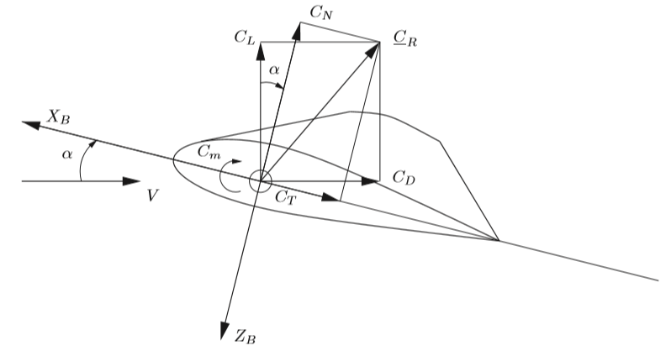
\includegraphics[width=0.5\linewidth]{figures/coordinates_converting_forces.png}
    \caption{Converting Aerodynamic Forces to Body Forces \cite{Timmer2024ProjectDesign}}
    \label{fig:forces_coordinate_transformation}
\end{figure}


\noindent where $\alpha$ is the angle of attack. Note that for small values of $\alpha$, the normal force is approximately equal to the aerodynamic lift.\\

\noindent A simplified visualization of the wing loading, as well as the coordinate system used for the calculation of the shear, bending and torsion, is showcased in \autoref{fig:candidate_coordinate_system}. For the purposes of this analysis, A distributed force $w(x)$ will be considered, as well as the engine weight $P_E$, located at $x_E$, and its corresponding bending moment $M_E$.

\begin{figure}[H]
    \centering
    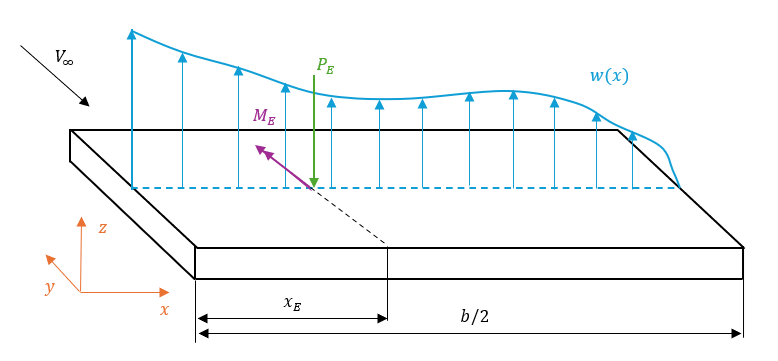
\includegraphics[width=0.5\linewidth]{beam_loading.png}
    \caption{Wing Loading Visualization}
    \label{fig:candidate_coordinate_system}
\end{figure}


\subsection*{Wing Sweep}
The planform design established in \textit{Wing Aerodynamic Design} \cite{Koppejan2024WingDesign} features a swept wing. Swept wings introduce complex load phenomena into the structure, which are outside of the scope of this course \cite{Timmer2024AE2111-IReader}. Therefore, a simpler shape will be considered for the construction of force and moment diagrams - an equivalent trapezoidal wing with a constant sweep angle (see: \autoref{fig:fd_assumptions_equivalent_unswept_wing}). The new model can be assumed to have the same values as the original wing, with the exception of the sweep at the flexural axis, which is reduced from the original sweep angle $\Lambda$ to zero \cite{Timmer2024AE2111-IReader}.
\begin{figure}[h]
    \centering
    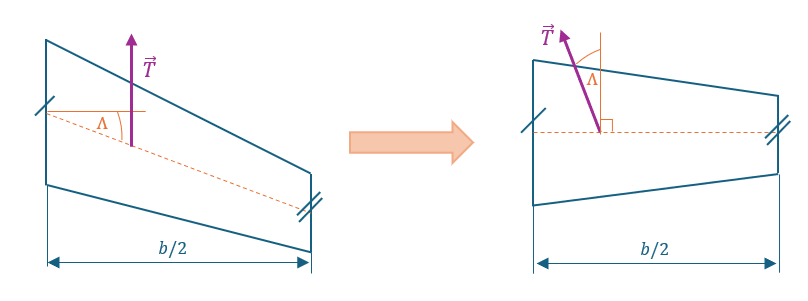
\includegraphics[width=0.85\linewidth]{figures/wing_sweep_effect.png}
    \caption{Equivalent unswept wing model}
    \label{fig:fd_assumptions_equivalent_unswept_wing}
\end{figure}

\noindent One consequence of this assumption is the changed direction of the thrust - as shown in \autoref{fig:fd_assumptions_equivalent_unswept_wing}, the orientation of the vector changes by an angle $\Lambda$. This happens because of the nature of the simplification - the whole planform is rotated to negate the effect of the sweep, and so is the thrust vector \cite{Timmer2024AE2111-IReader}.\\

\noindent The use of an equivalent trapezoidal wing is valid for modelling the variation of aerodynamic forces across the wing. However, it cannot be used in XFLR5 simulations, as the wing sweep affects the lift distribution, resulting in an overestimation of lift force towards the base of the wing, and an underestimation at the tips compared to the swept wing \cite{Timmer2024AE2111-IReader}.

\subsection*{In-Plane Forces and Moments}
The simplified loading case only considers shear forces in the vertical direction, i. e. perpendicular to the chord line. Therefore, the in-plane shear acting in the direction tangential to the chord line will be neglected. The same applies to bending moments - only those acting along the axis normal to the chord line are analyzed, and the in-plane bending of the wing box will not be regarded.\\

\noindent Neglecting the in-plane loads will, indispensably, lead to an overestimation of the performance of the wingbox in terms of strength and stiffness. In-plane interferences may lead to structural fatigue and shear fractures in metals \cite{Yin2015AMaterials}. However, the contribution of these loads to the shear, bending and torsion of the wingbox is negligible \cite{Timmer2024AE2111-IReader}, and hence, they are not considered in this part of the structural analysis.











%Note that formally speaking, point forces and couple moments can also be included in the distributed loading functions by use of Dirac-delta functions. However, for sake of simplicity, point forces and couple moments will be treated separately from the distributed load



\section{Aerodynamic Loading Analysis}  \label{sec:fd_aerodynamic_loading_analysis}
%Comment on the different reference frames for XFLR5 and force analysis [Fig. 9, p. 26 of the Reader].


\section{Shear Force, Bending Moment, and Torque}   \label{sec:fd_shear_moment_torque}
%Derivation of the shear force, bending moment and torque diagrams, and the corresponding plots. 

%Include two graphs for each plot: one corresponding to a critical load case with positive load factor found in WP4.3, and one corresponding to a critical load case with negative load factor found in WP4.3. Note that the inertial force on all elements depends on the load factor.
This section focuses on the formulae derivation and graphical representation of the shear force, bending moment, and torque acting on the wingbox. These are determined by the distributed aerodynamic loading, previously obtained in \autoref{sec:fd_aerodynamic_loading_analysis}.

\subsection*{Shear Force}
%shear force specific assumption
\noindent Adding to the general assumptions made above, the calculation of the shear force along the wing will only include the shear force contribution due to the lift distribution and none of the external force such as engine weight, fuel weight, and the weight of the wing itself. This assumption is deemed to be valid as it will cause a conservative estimation of the shear force. The shear force can be expressed in terms of the distributed loading as shown in \autoref{eq:shear_force_relation}

\begin{equation} \label{eq:shear_force_relation}
    w(x) = -\frac{dV}{dx}
\end{equation}
\noindent This expression can be integrated to obtain an expression for the shear force distribution along the wing as shown in \autoref{shear_force_integral}
\begin{equation} \label{shear_force_integral}
    V(x) = \int^L_x{w(x)dx}
\end{equation}

\subsection*{Bending Moment}
The bending moment $M$ is generally expressed as the second integral of the distributed load function, and hence closely related to the shear force $V$. It can be calculated by integrating \autoref{eq:fd:moment_shear_relation} \cite{Timmer2024AE2111-IReader} along the \textit{x}-axis.
\begin{equation}    \label{eq:fd:moment_shear_relation}
    V(x)=\frac{dM}{dx}
\end{equation}

\begin{comment}
Suppose a couple moment $M$ is applied at a location $x_2$ \todo{Would do nicely with a figure}. The bending moment at a given spanwise location $x$ can be expressed using \autoref{eq:fd_moment_at_x} \cite{Timmer2024AE2111-IReader}.
\begin{equation}    \label{eq:fd_moment_at_x}
   -M(x)=\int^L_x{V(x)dx}\space+M\left(1-u_{x_2}(x)\right)
\end{equation}
\noindent In this case, $u_{x_2}$ is the step function which attains a value of $0$ for $x<x_2$ and $1$ for $x\geq x_2$. In the case of an aircraft wing, a point moment would be a simplified representation of the bending relief provided by the engine weight $M_E$. The moment itself can be calculated as a product of the engine's weight $P_E$ and spanwise position $x_E$, i.e.:
\begin{equation*}
    M_E=P_E\cdot x_E
\end{equation*}

with $P_E$ and $x_E$ attaining the values of $(9630\cdot9.81)$ N and $9.37$ m, respectively, based on the results of propulsion system sizing from \textit{Further Aircraft Design} \cite{} \todo{cite WP3}. Substituting these values yields an engine bending relief moment $M_E$ of $885.187$ kNm.\\
\end{comment}
\noindent Since only the bending contributions of lift and engine weight are considered to act on the wing, and no additional bending moments are present in the load model, the internal bending moment $M$ at a given spanwise location $x$ can simply be evaluated as:
\begin{equation*}
    -M(x)=\int^{b/2}_x V(x)dx.
\end{equation*}



\subsection*{Torque}
% You may assume the shear centre to coincide with the centroid of the wing box cross section
For the torque, the shear center is required. Here, it can be assumed that the shear center coincides with the centroid of the wing box \cite{Timmer2024AE2111-IReader}, which is to be determined in \autoref{} \todo{cite section}. The loads of interest for the torque distribution are the lift distribution and the thrust force. The direction of the thrust force is pointed inward towards the fuselage as shown in \autoref{fig:fd_assumptions_equivalent_unswept_wing}. Therefore, to determine the torque, only the component of the thrust perpendicular to the shear center should be taken into account, using \autoref{fig:thrust_perpendicular}. 

\begin{equation}
    \label{fig:thrust_perpendicular}
    T_{\perp sc} = T\cos(\Lambda)
\end{equation}

\noindent The torsion at a location $x$ along the wing span can be determined using \autoref{eq:torsional_distribution}. In this equation, $L(x)$ is the function describing the distributed lift in the spanwise direction, $d(x)$ is the distance between the point of application of the distributed load and the shear centre, $d_1$ is the perpendicular distance between the orthogonal component of the thrust force T and the shear centre and $d_2$ is the distance between the application of the engine weight $W_E$ and the shear centre. $T_{\perp sc}$ is applied at position $x_1$, where the step function $u_{x_1}$ is equal to 0 for $x<x_1$ and 1 for $x\geq x_1$. $u_{x_2}$ behaves similar to this with the engine weight at $x_2$.

\begin{equation}
    \tau(x) = \int_x^{b/2}[L(x)d(x)]dx + T_{\perp sc}d_1 \left(1 - u_{x_1}(x) \right) - W_Ed_2\left(1 - u_{x_2}(x) \right)
    \label{eq:torsional_distribution}
\end{equation}

\noindent For the contribution of the weight of the engine to the internal torque distribution, the assumption is made that this load acts as a point force at the leading edge of the wing. This means that the distance $d_2$ is equal to the distance between the leading edge of the wing and the shear centre at the location $x_2$ along the shear centre. The engines are placed at $x_2 = 9.37$ m from the centre of the fuselage. The engine mass is equal to $9630$ kg. \\

\noindent The vertical distance between the shear centre and engine thrust is equal to $d_1$ and is to be determined when the centroid of the wing box is known. The spanwise location of the applied thrust is the same as for the weight of the engine and thus $x_1 = x_2 = 9.37$ m. The engine thrust is equal to $467.06$ kN. The sweep angle that is used in this equation is the half-chord sweep angle and is equal to $26.55$ deg.

\begin{equation}
    \tau(x) = \int_x^{31.36}[L(x)d(x)]dx + 467060 \cdot \cos{(26.55)} \cdot d_1 \left(1 - u_{9.37}(x) \right) - 9630 \cdot 9.81 \cdot d_2\left(1 - u_{9.37}(x) \right)
    \label{eq:torsional_distribution_with_numbers}
\end{equation}

\section{Explanation of Critical Cases} \label{sec:fd_critical_cases}
% Justification on why these load cases can be considered as the most critical
\chapter{Stiffness Calculation}
\label{ch:Stiff_Calc}



YOOOOOOO WAGWAN THIS IS SOME COOL PLACEHOLDER TEXT

\textcolor{orange}{I LOOOOOOVVVEEE it!! \\
    -The Burger King (Louisville, Kentucky 1407)\\
        -King Arthur (Came a lot, some castle 200 b.c.)\\
            -Cleopatra (Middle Earth, On a T-Rex 64 Million B.C.)}
\section{Assumptions made for stiffness calculations}
The loading of the wingbox has been determined, now the deflections can be calculated to find the structural and geometric requirements. The process for this can get quite complex, that is why some  assumptions will be made to simplify the calculations:
    In order to test the rigidity of the wing structure some simplifications needed to be made to properly be able to test it.
\begin{description}
    \item[Constant thickness throughout a plate] This can be done because most commercial plates have a singular thickness and choosing a thickness for every span position, would overcomplicate making the tool.

    \item[All load is carried by the wingbox] Using this assumption the wingbox will become stronger than the actual needed strength. This will make the loading used easier as it will be the exact numbers from \autoref{ch:ForceDiagram}.

    \item[Spar position is constant relative to chord length] This assumptions allows the the height of the spars to be linearly scaled with the chord. This will simplify the moment of inertia calculations for each spanwise point.

    \item[Stringer position in constant relative to chord length] This assumption will make sure that the stingers can will always be spaced in a way to prevent buckling. This way only the worst case of spacing needs to be considered.. 

    \item[All panels are constant with no cuts i.e. no 2 panels fastened] This assumption will allow for to use the equations provided by the reader, without having to considers points with a higher stress concentrations \cite{Timmer2024ProjectDesign}.
\end{description}
    
\section{Method}
In order to produce designs that met the required specifications, the procedure shown in \autoref{fig:sketch_designs_procedure} was followed. This process needed to be repeated for all the possible combinations of the parameters that are being analyzed. The designs that meet the requirements and will later be compared. The final choice will be made based on the mass of the design and the design philosophies.

\begin{figure}[H]
    \centering
    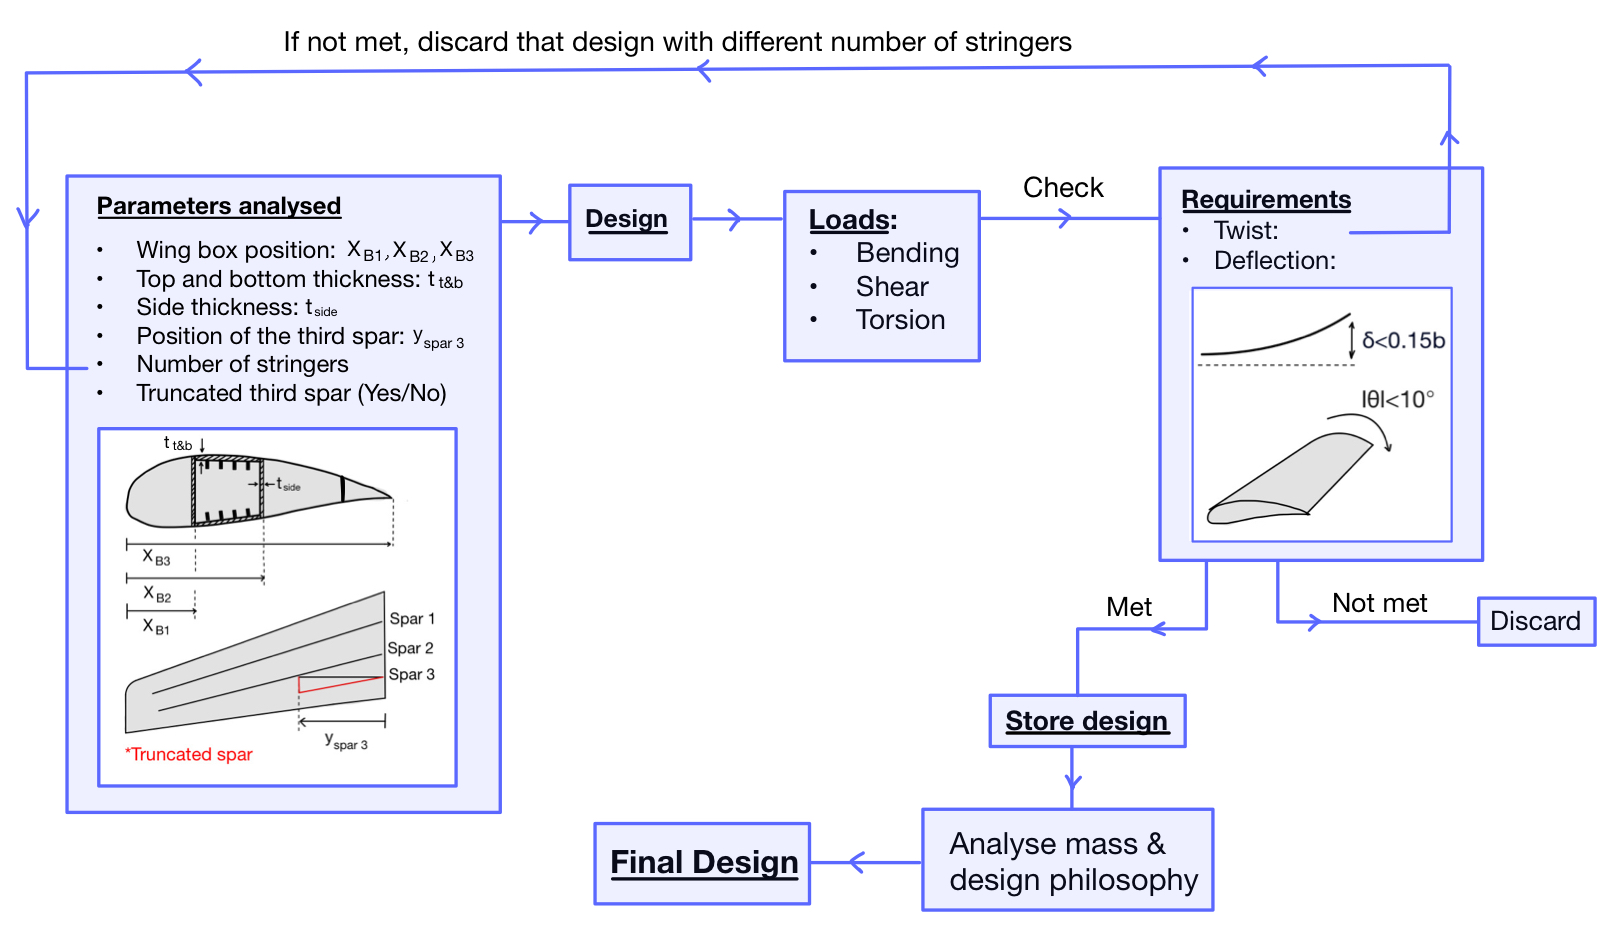
\includegraphics[width=1.1\linewidth]{figures/diagram python code.jpeg}
    \caption{Production of designs procedure}
    \label{fig:sketch_designs_procedure}
\end{figure}

\begin{itemize}
    \item Chordwise positioning of the spars 
    \item Thickness of the Spar caps 
    \item Thickness of the shear webs 
    \item Number of stringers 
    \item The spanwise end of the auxiliary, third spar 
    \item Whether the third spar is truncated or not. 
\end{itemize}
    from this we get the cross sectional area of the wingbox at all spanwise points

    2. using the cross section, get centroid, i.XX and i.YY 

    
\section{Results of the Python code}
\chapter{Preliminary Wing Box Design}
\label{ch:Prelim_WB_Des}
\noindent The wing box is the primary wing structure which serves as the base for all wing components. It needs to be designed in such a way that the whole wing will be able to cope/withstand all forces (bending, torsion, shear, etc.) acting on it during all parts of a flight. Firstly, the overview of the design procedure is presented in \autoref{sec:design procedure}. Secondly, the specific functions of the wing box will be stated in \autoref{sec:FuncAnalWinbox}. These functions were found based on calculations performed earlier in \autoref{ch:LoadAnalysis} and 
\autoref{ch:Design Analysis}. In \autoref{sec:Loading_Diagrams} six different V-n diagrams were derived from the specified conditions. Next in \autoref{sec:Tab_LoadCase} load cases are defined based on $\left(V_{EAS}-n\right)$ diagrams. These load cases are later used in \autoref{sec:Prelim_Des_Ops} to came up with three design options that meet the critical requirements stated earlier in \autoref{sec:Req_Anal_WB}.

\begin{comment}
    
One of these functions is being able to withstand the loads and moments determined in \autoref{ch:ForceDiagram}, while adhering to the critical requirements set in \autoref{ch:Stiff_Calc}. Those loads were found using the $\left(V_{EAS}-n\right)$ diagrams in \autoref{sec:Loading_Diagrams}. The diagrams then created the so-called load cases, where the loads on the wing box would be the highest. These specific scenarios are highlighted in \autoref{sec:Tab_LoadCase}. The requirements set in \autoref{ch:Stiff_Calc} will then in combination with the scenarios from \autoref{sec:Tab_LoadCase}, generate the final wing box requirements in \autoref{sec:Req_Anal_WB}. \autoref{sec:Prelim_Des_Ops} will then fulfill these requirements by generating three separate wing box designs.
\end{comment}

\section{Wing box design procedure}
\label{sec:design procedure}
Wing box design is a complicated and iterative process that requires the usage of tools obtained earlier in \autoref{ch:LoadAnalysis} and \autoref{ch:Design Analysis}. The first part of the design process is to obtain a manoeuvre-loading diagram for several flight cases to use them to define appropriate loading cases. These load cases along with force diagrams obtained earlier in \autoref{ch:LoadAnalysis} were used to define final critical requirements that directly influenced the design. At this point, all three designs could have been proposed. The design team came up with three designs (based on different philosophies) that were later checked with the tool obtained in \autoref{ch:Design Analysis} to meet the critical requirements. Finally, the process of checking the requirements along with optimizing the preliminary design was performed several times to get three designs that meet all the critical requirements stated earlier. The overview of the whole procedure is presented on the \autoref{fig:flowchart}.




\usetikzlibrary{shapes.geometric, arrows}



\definecolor{70af333d-4869-5f2a-97ca-9904a9fce6c3}{RGB}{179, 254, 174}
\definecolor{f3551e38-74df-57e2-b793-83d7fe876c85}{RGB}{0, 0, 0}
\definecolor{0b71a967-1f15-55a5-9bb9-70efa7b4fc58}{RGB}{51, 51, 51}
\definecolor{747aec21-333b-59ee-84e3-ddff893e5ccd}{RGB}{255, 216, 176}
\definecolor{adaee4ed-88c8-5b21-a9e7-31316ebef86f}{RGB}{255, 179, 178}
\definecolor{5856d031-3da1-575c-834e-c77e9e438c62}{RGB}{162, 177, 195}

\tikzstyle{WP2-diamond} = [diamond, minimum width=3cm, minimum height=2cm, text centered, font=\large, color=0b71a967-1f15-55a5-9bb9-70efa7b4fc58, draw=f3551e38-74df-57e2-b793-83d7fe876c85, line width=1, fill=70af333d-4869-5f2a-97ca-9904a9fce6c3]
\tikzstyle{V-n-Rectangle} = [rectangle, minimum width=3cm, minimum height=1cm, text centered, font=\normalsize, color=0b71a967-1f15-55a5-9bb9-70efa7b4fc58, draw=f3551e38-74df-57e2-b793-83d7fe876c85, line width=1, fill=747aec21-333b-59ee-84e3-ddff893e5ccd]
\tikzstyle{c1348099-d7cb-5a2d-89c5-daa2787c1591} = [rectangle, minimum width=3cm, minimum height=1cm, text centered, font=\normalsize, color=0b71a967-1f15-55a5-9bb9-70efa7b4fc58, draw=f3551e38-74df-57e2-b793-83d7fe876c85, line width=1, fill=747aec21-333b-59ee-84e3-ddff893e5ccd]
\tikzstyle{512bdd77-c3aa-5669-a956-85f7a90c6fb4} = [rectangle, rounded corners, minimum width=3cm, minimum height=1cm, text centered, font=\normalsize, color=0b71a967-1f15-55a5-9bb9-70efa7b4fc58, draw=f3551e38-74df-57e2-b793-83d7fe876c85, line width=1, fill=adaee4ed-88c8-5b21-a9e7-31316ebef86f]
\tikzstyle{7be24b85-97d0-5b76-ba9e-d94005dca8f2} = [thick, draw=5856d031-3da1-575c-834e-c77e9e438c62, line width=2, ->, >=stealth]


\begin{figure}[H]
    \centering
\begin{tikzpicture}[node distance=2cm]

\node (5ad49ccc-6515-4d1c-b24b-cd30eb88c845) [V-n-Rectangle, below of=9214c975-5b8d-40a1-a919-5f0ca9435a02, yshift=-0.5cm] {V-n Diagrams};
\node (9214c975-5b8d-40a1-a919-5f0ca9435a02) [WP2-diamond, above of=5ad49ccc-6515-4d1c-b24b-cd30eb88c845, xshift=4cm] {WP 4.1};
\node (d15626ae-577c-46b5-ab8e-b609b527d898) [WP2-diamond, right of=9214c975-5b8d-40a1-a919-5f0ca9435a02, xshift=2cm] {WP 4.2};

\node (77d529d5-6f80-4ba7-852d-5db0a8bfabfe) [V-n-Rectangle, right of=5ad49ccc-6515-4d1c-b24b-cd30eb88c845, xshift=2cm] {Load Cases};
\node (2781bf06-b5d3-47c0-a90f-68879a683784) [c1348099-d7cb-5a2d-89c5-daa2787c1591, right of=5ad49ccc-6515-4d1c-b24b-cd30eb88c845, xshift=6cm] {Critical Requirements};
\node (9b8095fe-e9a2-4d7b-95f7-1b296a4bc41f) [512bdd77-c3aa-5669-a956-85f7a90c6fb4, right of=5ad49ccc-6515-4d1c-b24b-cd30eb88c845, xshift=10cm] {Three Designs};
\node (46582238-2501-40fd-9703-900311286e92) [V-n-Rectangle, below of=5ad49ccc-6515-4d1c-b24b-cd30eb88c845, xshift=10cm] {CHECK!};
\draw [7be24b85-97d0-5b76-ba9e-d94005dca8f2] (77d529d5-6f80-4ba7-852d-5db0a8bfabfe) --  (2781bf06-b5d3-47c0-a90f-68879a683784);
\draw [7be24b85-97d0-5b76-ba9e-d94005dca8f2] (5ad49ccc-6515-4d1c-b24b-cd30eb88c845) --  (77d529d5-6f80-4ba7-852d-5db0a8bfabfe);
\draw [7be24b85-97d0-5b76-ba9e-d94005dca8f2] (2781bf06-b5d3-47c0-a90f-68879a683784) --  (9b8095fe-e9a2-4d7b-95f7-1b296a4bc41f);
\draw [7be24b85-97d0-5b76-ba9e-d94005dca8f2] (9214c975-5b8d-40a1-a919-5f0ca9435a02) --  (77d529d5-6f80-4ba7-852d-5db0a8bfabfe);
\draw [7be24b85-97d0-5b76-ba9e-d94005dca8f2] (d15626ae-577c-46b5-ab8e-b609b527d898) --  (2781bf06-b5d3-47c0-a90f-68879a683784);
\draw [7be24b85-97d0-5b76-ba9e-d94005dca8f2] (9b8095fe-e9a2-4d7b-95f7-1b296a4bc41f) |-  (46582238-2501-40fd-9703-900311286e92);
\draw [7be24b85-97d0-5b76-ba9e-d94005dca8f2] (46582238-2501-40fd-9703-900311286e92) -|  (2781bf06-b5d3-47c0-a90f-68879a683784);
\end{tikzpicture}
    \caption{Wing box design procedure visualisation}
    \label{fig:flowchart}
\end{figure}


\section{Wing Box Functional Analysis}
\label{sec:FuncAnalWinbox}
\autoref{tab:Wingbox_functions} presents the main functionalities that a wing box should provide. All of them were taken into account during the iterative design process.

\begin{table}[H]
    \centering
    \caption{Functions of a Wing box}
    \begin{tabularx}{\textwidth}{|p{.2\textwidth} |p{.745\textwidth}|}
        \hline
        \cellcolor{blue!15}\textbf{Code} & \cellcolor{blue!15}\textbf{Function} \\
        \hline

        \cellcolor{blue!15} FUN-BOX-01 & \textit{Provide a load-bearing structure to the wing.}\\
        \hline
        \cellcolor{blue!15} FUN-BOX-02 & \textit{Provide structural rigidity to the wing.}\\
        \hline
        \cellcolor{blue!15} FUN-BOX-03 & \textit{House the fuel stored in the wing.}\\
        \hline
        \cellcolor{blue!15} FUN-BOX-04 & \textit{Provide a way to attach the Control Surfaces to the wing.}\\
        \hline
        \cellcolor{blue!15} FUN-BOX-05 & \textit{Provide housing and protection for the electronics in the wing.}\\
        \hline
        \cellcolor{blue!15} FUN-BOX-06 & \textit{Provide extra resistance to flutter.}\\
        \hline
        \cellcolor{blue!15} FUN-BOX-07 & \textit{TBD}\\
        \hline
        \cellcolor{blue!15} FUN-BOX-08 & \textit{TBD}\\
        \hline
        
        
    \end{tabularx}
      
        \label{tab:Wingbox_functions}
\end{table}
\todo{remove the final 2 if we cannot think of others}
\section{Manoeuvre Loading Diagram}
\label{sec:Loading_Diagrams}

\noindent Finding the load cases requires drawing the manoeuvre loading diagram, also called V-n diagram, for different altitudes and weights considered. This graph shows which load factors correspond to the aircraft's most characteristic speeds. Here six different V-n diagrams will be provided by analysing the aircraft flying at cruise and sea altitude at the following three weight configurations: OEW, OEW + MPW, and OEW + MPW + MF such that MTOW is obtained. \autoref{fig:v-ncaseCrit} shows the most critical V-n diagram which corresponded to... \autoref{v-n_diagrams} contains the other five V-n diagrams. To draw these diagrams the following characteristic velocities and loading factors were used:

\begin{itemize}
    \item $V_{S0}$: stall speed with flaps extended. \autoref{eq:v_so}, taken from \textit{"AE2111-I: System Design - Project Reader" } \cite{Timmer2024AE2111-IReader}, was used. Here $W$ was replaced for each one of the weights in the three cases, $\rho$ corresponds to the sea level or cruise density, depending on the case being analysed, $C_{L_{max _{land}}}$ has a value of $2.5$, and the surface area of the wing (denoted by $S$) is $265.21$ m$^2$. %add reference to our previous report (report III)
    \begin{equation}
    \label{eq:v_so}
        V_{S0} = \sqrt{\frac{2W}{C_{L_{max _{land}}} \rho S}} 
    \end{equation}
    \item $V_{S1}$: stall speed with flaps retracted. \autoref{V_s1} \cite{Timmer2024AE2111-IReader} was used in this case. Variables in this equation are the same as the ones mentioned for $V_{S0}$, the only changing parameter is $C_{L_{max _{clean}}}$, which takes a value of $1.7$.
    \begin{equation}
    \label{V_s1}
         V_{S1} = \sqrt{\frac{2W}{C_{L_{max _{clean}}} \rho S}}
    \end{equation}
    \item $V_A$: manoeuvring speed. This was calculated by using \autoref{v_a} \cite{Timmer2024AE2111-IReader}. The variables in this equation are again the same as the ones used for $V_{S0}$. The new variable is $n_{max}$ which corresponds to a value of $2.5$ in the cases being analysed. 
    \begin{equation}
    \label{v_a}
        V_A = \sqrt{\frac{2n_{max}W}{C_{L_{max_{clean}}}S\rho}}
    \end{equation}
    \item $V_C$: cruise speed. This was given to be 241.96 ms$^{-1}$ \cite{Timmer2024AE2111-IReader}.
    \item $V_D$: design dive speed. The calculation for this speed can be directly calculated by using \autoref{v_d} \cite{Timmer2024AE2111-IReader}.
    \begin{equation}
    \label{v_d}
        V_D = 1.5V_C
    \end{equation}
    
    \item $V_F$: design wing-flap speed. This parameter was calculated by choosing the highest velocity out of: $1.6V_{s1}$, $1.8V_{s1}$, $1.8V_{s0}$ and $V_{intersect}$, which was calculated by multiplying $V_{s1}$ by $\sqrt{2}$.
    
    \item $n_{max}$: positive limit manoeuvring load factor. This value may not be less than $2.5$ or higher than $3.8$. It can be calculated by using \autoref{n_max} \cite{Timmer2024AE2111-IReader}. For all of the considered cases, $n_{max}$ was lower than $2.5$, therefore $n_{max}$ resulted in a value of $2.5$ for all cases. 
    \begin{equation}
    \label{n_max}
        n_{max} = 2.1 + \frac{24000}{W+10000}
    \end{equation}
    
    \item $n_{min}$: negative limit for manoeuvring load factor. This value could not be less than $-1$. Therefore this was the assumed value for all cases \cite{Timmer2024AE2111-IReader}.
    \item The maximum load factor with flaps deflected was assumed to be $2.0$, according to \textit{"AE2111-I: System Design - Project Reader" } \cite{Timmer2024AE2111-IReader}.
\end{itemize}

\begin{figure}[H]
    \centering
    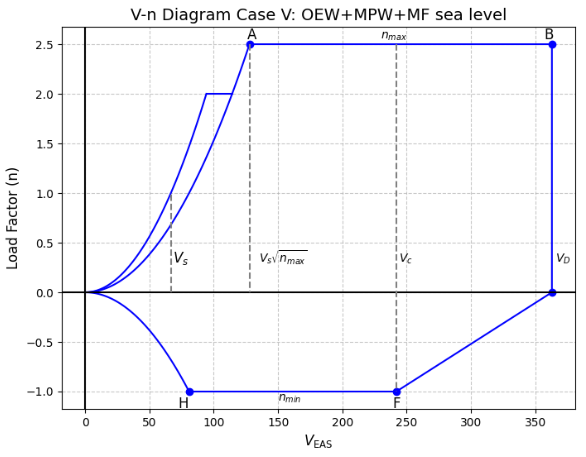
\includegraphics[width=0.65\linewidth]{figures/v-n diagram case V.png}
    \caption{V-n diagram for the aircraft operating at OEW, MPW and MF; at sea level conditions} 
    \label{fig:v-ncaseCrit}
\end{figure}

\section{Table of Load Cases}
\label{sec:Tab_LoadCase}
As six different manoeuvre loading diagrams were obtained in the previous section (\autoref{sec:Loading_Diagrams}), they can be used to develop appropriate load cases that will later be used to define critical design requirements. By looking at \autoref{fig:v-ncaseCrit} five critical load cases can be found for each one of the V-n diagrams:
%add reference to any V-n diagram
\begin{itemize}
    \item Point A: This point represents the maximum load factor $n_{max}$ the aircraft can experience at the manoeuvring speed ($V_A$). If the load factor is further increased the aircraft will experience structural damage.
    \item Point B: This is the maximum positive load factor at the design dive speed $V_D$, for safety reasons, the aircraft cannot overpass this limit. 
    \item Point F: Corresponds to the minimum load factor the aircraft can handle at cruise speed ($V_c$). 
    \item Point H: This load case corresponds to the minimum load factor the aircraft can experience, corresponding to $V_{s1}$.
    \item Horizontal intersection at n = $2$: Maximum load factor the aircraft can handle with flaps down.
\end{itemize}

\noindent These load cases are then shown for each combination of Weight and Altitude considered. The results obtained are shown in \autoref{tab:LoadCases}.



\begin{longtable}{|>{\columncolor{blue!15}}c|p{3.2cm}|p{2cm}|c|c|c|p{2.6cm}|}
\caption{Table of considered Load Cases}
\label{tab:LoadCases}
\endfirsthead
    \hline
    \rowcolor{blue!15} \textbf{Load Case} & \textbf{Description} & \textbf{Speed$_{EAS}$ [m s$^-1$]} & \textbf{Altitude} & \textbf{Weight [kN]} & \textbf{n} & \textbf{Comments} \\
    \hline
    LC-1 & OEW Sea Level at $V_{d}$ & 362.94 & FL0 & 770.1 & 2.5 & Trimmed HLDs (clean config.) \\
    \hline
    LC-2 & OEW Sea Level at $V_{c}$ & 241.96 & FL0 & 770.1 & -1 & Trimmed HLDs (clean config.) \\ 
    \hline
    LC-3 & OEW Sea Level at $V_{f,intersection}$ & 74.68 & FL0 & 770.1 & 2 & This is with full flaps \\ \hline
    LC-4 & OEW Sea Level at $V_{a}$ & 83.50 & FL0 & 770.1 & 2.5 & Trimmed HLDs (clean config.) \\ 
    \hline
    LC-5 & OEW Sea Level at $V_{S1}$ & 52.81 & FL0 & 770.1 & -1 & Trimmed HLDs (clean config.) \\ 
    \hline
    LC-6 & OEW Cruise Level at $V_{d}$ & 184.47 & FL390 & 770.1 & 2.5 & Trimmed HLDs (clean config.) \\ 
    \hline
    LC-7 & OEW Cruise Level at $V_{c}$ & 122.98 & FL390 & 770.1 & -1 & Trimmed HLDs (clean config.) \\ 
    \hline
    LC-8 & OEW Cruise Level at $V_{f,intersection}$ & 74.68 & FL390 & 770.1 & 2 & This is with full flaps \\ 
    \hline
    LC-9 & OEW Cruise Level at $V_{a}$ & 83.50 & FL390 & 770.1 & 2.5 & Trimmed HLDs (clean config.) \\ 
    \hline
    LC-10 & OEW Cruise Level at $V_{S1}$ & 52.81 & FL390 & 770.1 & -1 & Trimmed HLDs (clean config.) \\ 
    \hline
    LC-11 & OEW+MPW Sea Level at $V_{d}$ & 362.94 & FL0 & 1040.6 & 2.5 & Trimmed HLDs (clean config.) \\ 
    \hline
    LC-12 & OEW+MPW Sea Level at $V_{c}$ & 241.96 & FL0 & 1040.6& -1 & Trimmed HLDs (clean config.) \\ 
    \hline
    LC-13 & OEW+MPW Sea Level at $V_{f,intersection}$ & 86.81 & FL0 & 1040.6 & 2 & This is with full flaps \\ 
    \hline
    LC-14 & OEW+MPW Sea Level at $V_{a}$ & 97.06 & FL0 & 1040.6 & 2.5 & Trimmed HLDs (clean config.) \\
    \hline
    LC-15 & OEW+MPW Sea Level at $V_{S1}$ & 61.39 & FL0 & 1040.6& -1 & Trimmed HLDs (clean config.) \\ 
    \hline
    LC-16 & OEW+MPW Cruise at $V_{d}$ & 184.47 & FL390 & 1040.6& 2.5 & Trimmed HLDs (clean config.) \\ 
    \hline
    LC-17 & OEW+MPW Cruise at $V_{c}$ & 122.98 & FL390 & 1040.6 & -1 & Trimmed HLDs (clean config.) \\ 
    \hline
    LC-18 & OEW+MPW Cruise at $V_{f,intersection}$ & 86.81 & FL390 & 1040.6 & 2 & This is with full flaps \\ 
    \hline
    LC-19 & OEW+MPW Cruise at $V_{a}$ & 97.06 & FL390 & 1040.6 & 2.5 & Trimmed HLDs (clean config.) \\ 
    \hline
    LC-20 & OEW+MPW Cruise at $V_{S1}$ & 61.39 & FL390 & 1040.6 & -1 & Trimmed HLDs (clean config.) \\ 
    \hline
    LC-21 & OEW+MPW+fuel Sea Level at $V_{d}$ & 362.94 & FL0 & 1803.4 & 2.5 & Trimmed HLDs (clean config.) \\ 
    \hline
    LC-22 & OEW+MPW+fuel Sea Level at $V_{c}$ & 241.96 & FL0 & 1803.4 & -1 & Trimmed HLDs (clean config.) \\ 
    \hline
    LC-23 & OEW+MPW+fuel Sea Level at $V_{f,intersection}$ & 114.29 & FL0 & 1803.4 & 2 & This is with full flaps \\ 
    \hline
    LC-24 & OEW+MPW+fuel Sea Level at $V_{a}$ & 127.78 & FL0 & 1803.4 & 2.5 & Trimmed HLDs (clean config.) \\ 
    \hline
    LC-25 & OEW+MPW+fuel Sea Level at $V_{S1}$ & 80.81 & FL0 & 1803.4 & -1 & Trimmed HLDs (clean config.) \\ 
    \hline
    LC-26 & OEW+MPW+fuel Cruise at $V_{d}$ & 184.47 & FL390 & 1803.4 & 2.5 & Trimmed HLDs (clean config.) \\ 
    \hline
    LC-27 & OEW+MPW+fuel Cruise at $V_{c}$ & 122.98 & FL390 & 1803.4 & -1 & Trimmed HLDs (clean config.) \\ 
    \hline
    LC-28 & OEW+MPW+fuel Cruise at $V_{f,intersection}$ & 114.29 & FL390 & 1803.4 & 2 & This is with full flaps \\ 
    \hline
    LC-29 & OEW+MPW+fuel Cruise at $V_{a}$ & 127.78 & FL390 & 1803.4 & 2.5 & Trimmed HLDs (clean config.) \\ 
    \hline
    LC-30 & OEW+MPW+fuel Cruise at $V_{S1}$ & 80.81 & FL390 & 1803.4 & -1 & Trimmed HLDs (clean config.) \\ 
    \hline
\end{longtable}
\todo{Decimal points are unrealistically accurate}


\section{Requirement Analysis}
\label{sec:Req_Anal_WB}
Out of 30 Load Cases presented in \autoref{tab:LoadCases} only a few of them will define critical load requirements that the design will be based on. These load cases could be obtained using both qualitative and numerical reasoning.
\newline
The qualitative approach is based on assuming that for the highest airplane weight (OEW + MPW + fuel) the highest lift is needed thus that loading case will be critical. Load cases from 21 - 30 all assume the highest airplane weight but on different flight levels. Out of these ten load cases, we select those with both the highest (2.5) and lowest (-1) load factors while ignoring cases with extended HLD (according to project reader \cite{Timmer2024AE2111-IReader}). This procedure led to the selection of four critical loading cases (LC-21, LC-22, LC-26, LC-27) which were used to define critical requirements presented in \autoref{tab:req_list_wingbox}.
\newline
The numerical method was earlier described in \autoref{ch:Design Analysis} and it will serve as confirmation of the after-mentioned qualitative approach.

\begin{comment}
    
After having obtained the most critical load cases in \autoref{sec:fd_critical_cases}, it is now possible to derive from them a requirements list for the wing box of the aircraft. This list is shown in \autoref{tab:req_list_wingbox}.
\end{comment}

\begin{longtable}[H]{|>{\columncolor{blue!15}}p{.2\textwidth} |p{.75\textwidth}|}
    \caption{Requirements list for the Wing box}
    \label{tab:req_list_wingbox}
    \endfirsthead
        \hline
        \textbf{Code} & \cellcolor{blue!15}\textbf{Function} \\
        \hline

         REQ-BOX-01-a & \textit{The wing tip shall not displace more than 15 \% of the wingspan when subjected to a load factor of $2.5$, whilst flying at an equivalent airspeed of $362.94$ ms $^{-1}$ at FL0, with maximum payload and no fuel, with all control surfaces retracted}\\
        \hline
         REQ-BOX-01-b & \textit{The wing tip shall not rotate more than $\pm 10 \degree $ of the wingspan when subjected to a load factor of $2.5$, whilst flying at an equivalent airspeed of $362.94$ ms $^{-1}$ at FL0, with maximum payload and no fuel, with all control surfaces retracted}\\
        \hline
        REQ-BOX-02-a & \textit{The wing tip shall not displace more than 15 \% of the wingspan when subjected to a load factor of $-1$, whilst flying at an equivalent airspeed of $241.96$ ms$^{-1}$ at FL0, with maximum payload and no fuel, with all control surfaces retracted}\\
        \hline
        REQ-BOX-02-b & \textit{The wing tip shall not rotate more than $\pm 10 \degree $ of the wingspan when subjected to a load factor of $2.5$, whilst flying at an equivalent airspeed of $241.96$ ms$^{-1}$ at FL0, with maximum payload and no fuel, with all control surfaces retracted}\\
        \hline
        REQ-BOX-03-a & \textit{The wing tip shall not deflect more than 15 \% of the wingspan when subjected to a load factor of $2.5$, whilst flying at an equivalent airspeed of $184.47$ ms$^{-1}$ at FL390, with maximum payload and no fuel, with all control surfaces retracted}\\
        \hline
        REQ-BOX-03-b & \textit{The wing tip shall not rotate more than $\pm 10 \degree $, when subjected to a load factor of $2.5$, whilst flying at an equivalent airspeed of $184.47$ ms$^{-1}$ at FL390, with maximum payload and full fuel, with all control surfaces retracted}\\
        \hline
        REQ-BOX-04-a & \textit{The wing tip shall not deflect more than 15 \% of the wingspan when subjected to a load factor of $-1$, whilst flying at an equivalent airspeed of $122.98$ ms$^{-1}$ at FL390, with maximum payload and full fuel, with all control surfaces retracted}\\
        \hline
        REQ-BOX-04-b & \textit{The wing tip shall not rotate more than $\pm 10 \degree $, when subjected to a load factor of $-1$, whilst flying at an equivalent airspeed of $122.98$ ms$^{-1}$ at FL390, with maximum payload and full fuel, with all control surfaces retracted}\\
        \hline
\end{longtable}

\section{Preliminary Design Options}
\label{sec:Prelim_Des_Ops}
This section will focus on the preliminary design of the wing box. Three different wing box designs will be selected. All of them will meet the requirements determined in \autoref{sec:Req_Anal_WB}. 

\noindent As \autoref{fig:flowchart} showed, the possible designs for the wing box structure will be found by making use of the forces and load cases found in \autoref{ch:LoadAnalysis} and the stiffness calculations provided in \autoref{ch:Design Analysis}. By combining the code developed in the previous two chapters a high number of design options for the wing box was obtained. Three designs needed to be selected, therefore design philosophies needed to be defined to refine the selection. These different design philosophies will be explained in the following sections, together with a picture of the resulting selected design.


%\noindent The use of strong spars that carry most of the bending loads will help simplify the complexity of the design. However in this case the material was set to be AL2024-T81, therefore spars cannot be strengthened by used a different material. If this restriction did not exist, it would be recommended to consider other options. Another way to counteract this constrain would be increasing the thickness of the skin. The bad part of this solution would be the increase in weight and price of the design, as more material is being used. \\

%\noindent A second option to increase the stiffness of the wing box is to place a high number of closely-spaced stringers. With this design the load will be more evenly distributed, and therefore its stiffness will increase. The downside of this option is that it increases the complexity of the design, and therefore manufacturing will increase the cost. \\

%\noindent Another option to meet the torsional stiffness requirement is the use of several closed cells within the wing box. This design rapidly increases the stiffness, however complexity and weight will also increase. Alternatively the use of truss-like structures shall also be considered. If the geometry is optimized, the structure will flexible and capable of sustaining high loads while maintaining a low weight. 

\subsection*{Design for Minimum Weight}
The first out of three preliminary designs will be based on the weight minimization philosophy. The main goal of this design is to meet all required conditions for deflection and rotation (described in \autoref{ch:Design Analysis}). Worth mentioning is the fact that this particular design is the current most optimal one but several factors such as buckling analysis or wing box damage tolerance were omitted until this point, thus it is very likely that this design might change when performing a more precise analysis. The cross-section of the design is presented on \autoref{fig:min_weight}. In this figure the blue lines represent the wingbox with the blue dots being the stingers.

\begin{figure}[H]
    \centering
    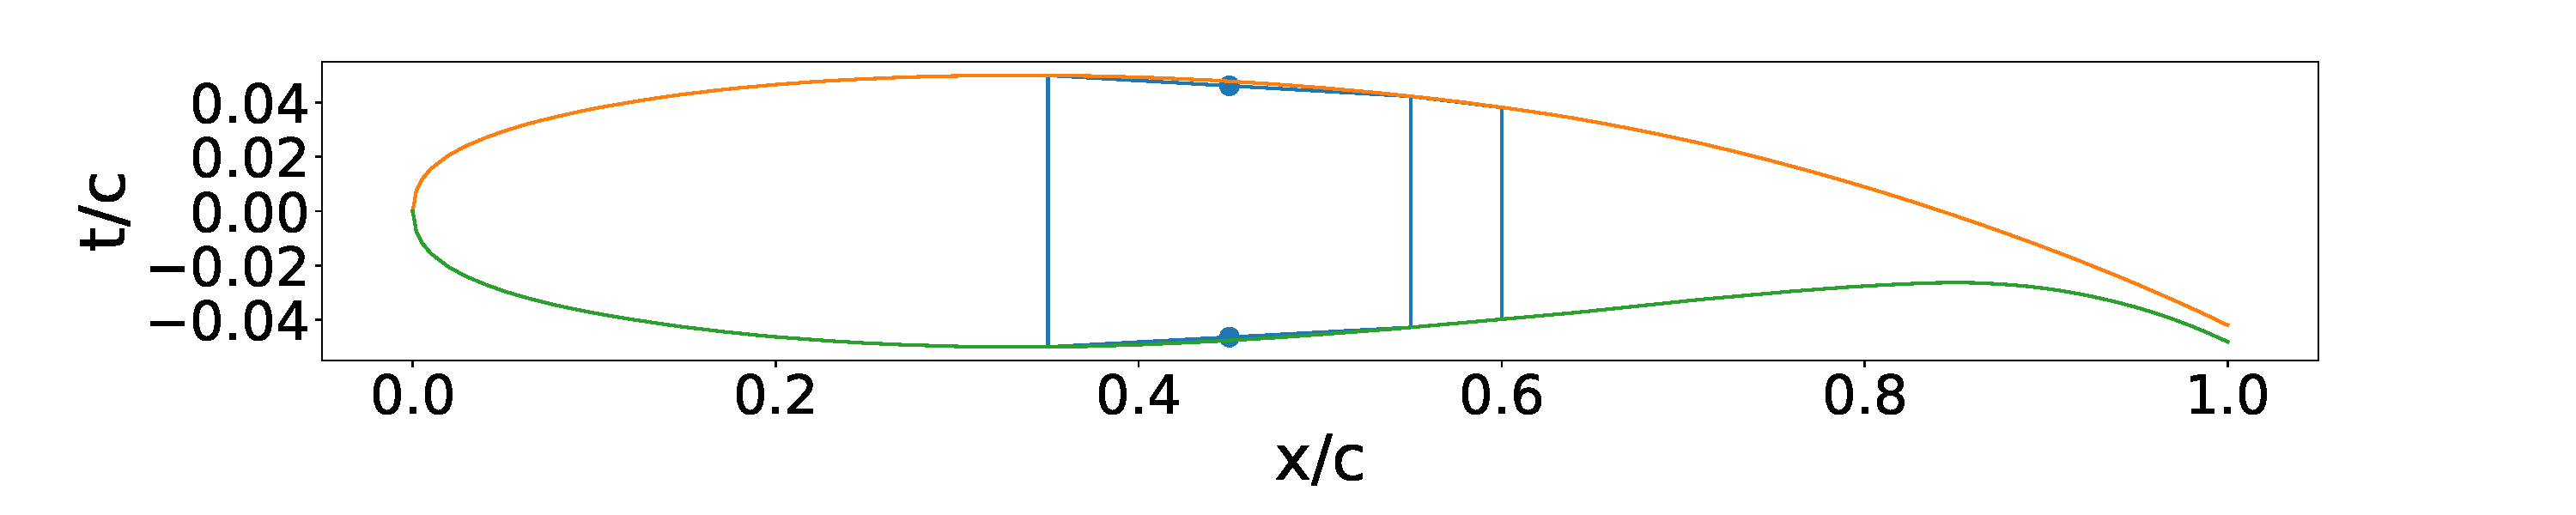
\includegraphics[width=0.9\linewidth]{figures/Cross_section_min_W.pdf}
    \caption{Cross section for the design optimized for minimum weight}
    \label{fig:min_weight}
\end{figure}

\subsection*{Design for Limit Load}
The second preliminary design will be designed towards the limit load, but it will be specifically designed towards minimizing buckling. This will be done by increasing the amount of stringers. The stringers increase the buckling resistance by decreasing the stringer spacing within the wingbox \cite{Timmer2024Project5}. This does however increase the weight significantly with respect to designs one and two.\\
The stingers are positioned only in the front cell of the wingbox and are evenly spaced throughout the box. The full geometry of the cross-section can be seen in \autoref{fig:limit_load_design}. In this figure the blue lines represent the wingbox with the blue dots being the stingers.
\begin{figure}[H]
    \centering
    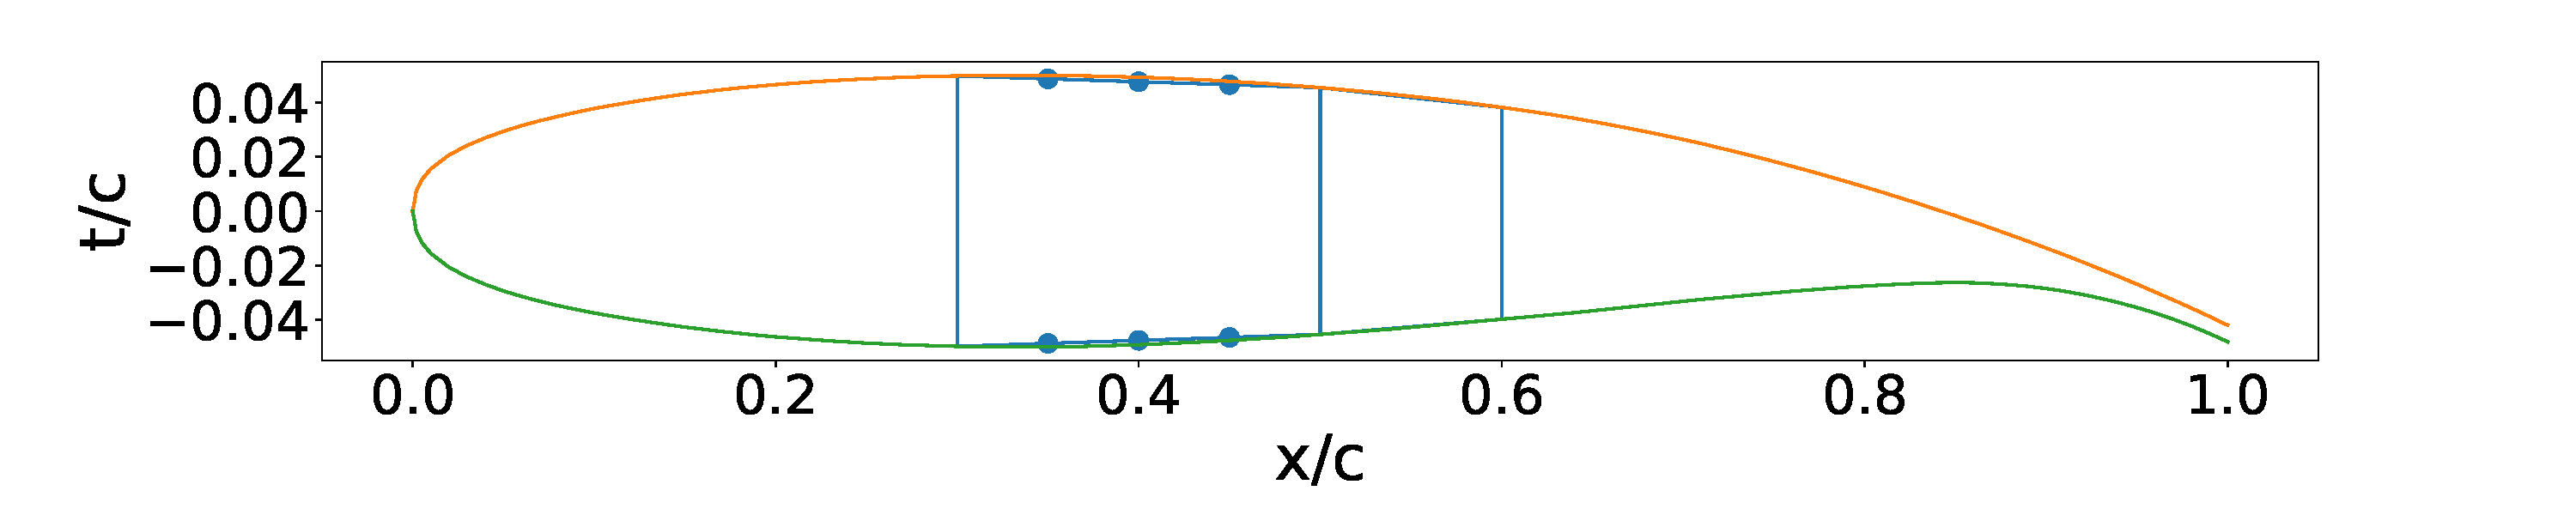
\includegraphics[width=0.9\linewidth]{figures/Cross_section_lim_load.pdf}
    \caption{Cross section for the design optimized for the limit load}
    \label{fig:limit_load_design}
\end{figure}

\subsection*{Design for Ultimate Load}
The third preliminary design optimizes for the ultimate load, which corresponds to $1.5$ times the limit load \cite{S.Bart2023UltimateLoad}. This ultimate load represents the maximum load the wing box must withstand during extreme conditions, ensuring the safety of the mission. The FAA mandates a safety factor of $1.5$ for prescribed limit loads, which are considered external loads on the structure\cite{2023FAARegulations}, this is specified in CFR 14, part 25.303. Therefore, designing for the ultimate load meets regulatory requirements and guarantees structural safety.

\noindent Additionally, this design aims to minimise weight, a key consideration in aerospace engineering. This explains why the number of stringers, represented by the two dots on the skin of the airfoil, is two. However, this design choice may have to be revisited during the future the future study of buckling behavior of the structure. as the design's stability under compressive loads was not yet examined.

\begin{figure}[H]
    \centering
    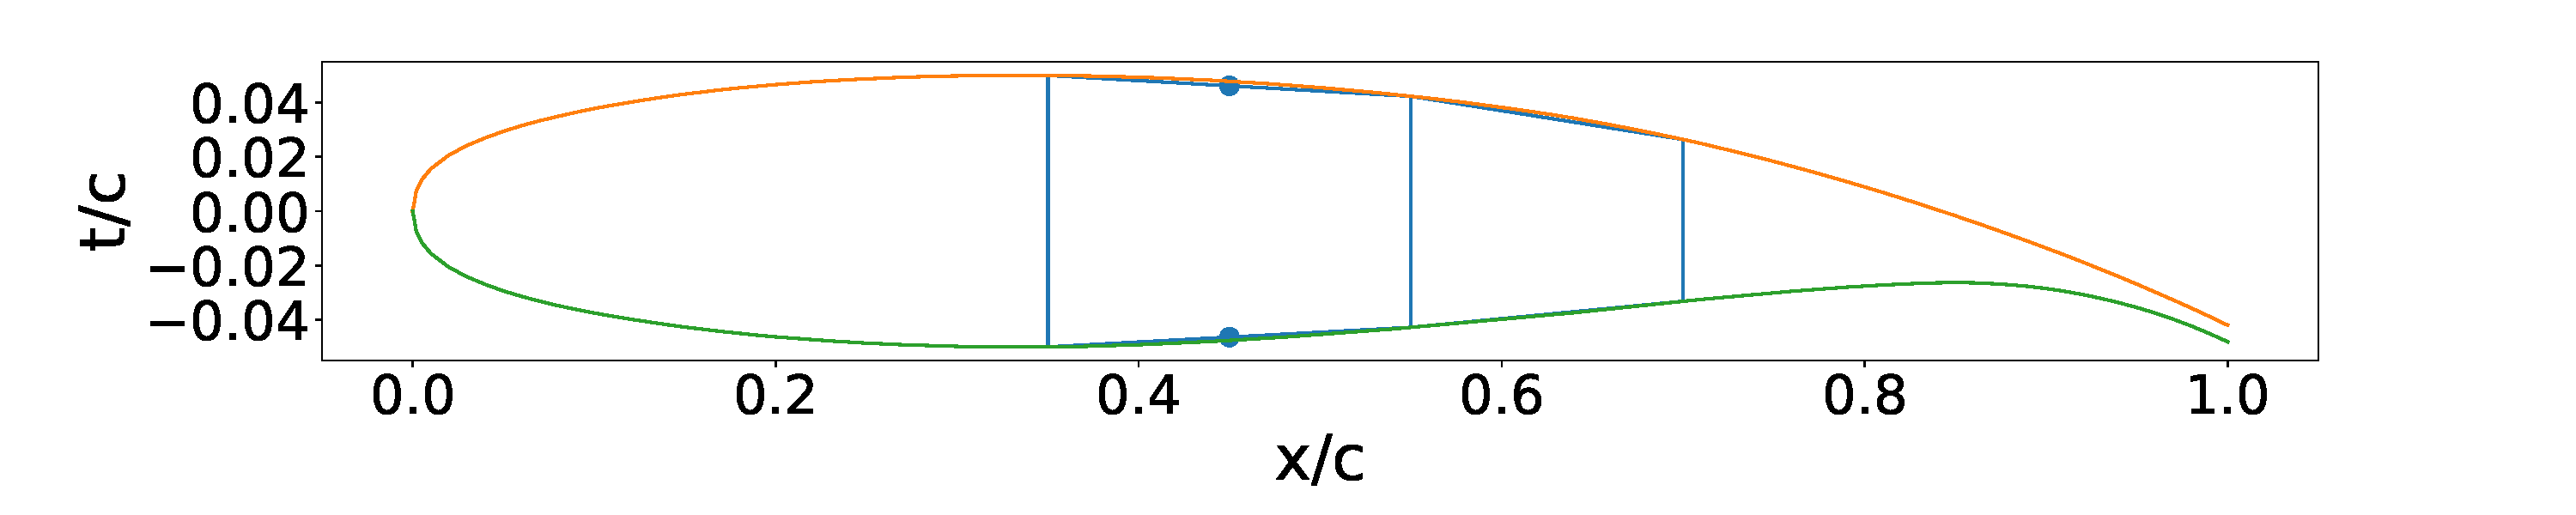
\includegraphics[width=0.9\linewidth]{figures/Cross_section_ult_load.pdf}
    \caption{Cross section for the design optimized for the ultimate load}
    \label{fig:ult_load_design}
\end{figure}

\subsection*{Design Parameter Table}
\autoref{tab:parameters_3_designs} shows the main geometrical parameters needed to fully describe the geometry of the three selected wing box designs. As previously explained, those values were calculated by making use of the code developed in \autoref{ch:LoadAnalysis}, \autoref{ch:Design Analysis} and the critical load cases found with the V-n diagrams generated at the beginning of this section. 

\begin{longtable}[c]{l|l|l|l|}
\caption{Parameters for the three selected designs}
\label{tab:parameters_3_designs}\\
\cline{2-4}
 &
  \cellcolor[HTML]{CBCEFB}\textbf{Design 1} &
  \cellcolor[HTML]{CBCEFB}\textbf{Design 2} &
  \cellcolor[HTML]{CBCEFB}\textbf{Design 3} \\ \hline
\endfirsthead
%
\multicolumn{4}{c}%
{{\bfseries Table \thetable\ continued from previous page}} \\
\cline{2-4}
 &
  \cellcolor[HTML]{CBCEFB}\textbf{Design 1} &
  \cellcolor[HTML]{CBCEFB}\textbf{Design 2} &
  \cellcolor[HTML]{CBCEFB}\textbf{Design 3} \\ \hline
\endhead
%
\multicolumn{1}{|l|}{\cellcolor[HTML]{CBCEFB}Main Design Philosophy} &
  Minimum weight &
  Ultimate load &
  Limit Load \\ \hline
\multicolumn{1}{|l|}{\cellcolor[HTML]{CBCEFB}Thickness top and bottom {[}m{]}} & 0.001  & 0.001  & 0.001  \\ \hline
\multicolumn{1}{|l|}{\cellcolor[HTML]{CBCEFB}Thickness sides {[}m{]}}          & 0.0007 & 0.0012 & 0.0007 \\ \hline
\multicolumn{1}{|l|}{\cellcolor[HTML]{CBCEFB}Number of stringers {[}-{]}}      & 2      & 2      & 6      \\ \hline
\multicolumn{1}{|l|}{\cellcolor[HTML]{CBCEFB}Mass {[}kg{]}}                    & 547.83 & 632    & 675.6  \\ \hline
\multicolumn{1}{|l|}{\cellcolor[HTML]{CBCEFB}Critical tip deflection {[}m{]}}                   & 3.62   & 3.39   & 2.78   \\ \hline
\multicolumn{1}{|l|}{\cellcolor[HTML]{CBCEFB}Critical tip twist {[}deg{]}}     & 8.2656 & 6.601  & 7.8064 \\ \hline
\multicolumn{1}{|l|}{\cellcolor[HTML]{CBCEFB}Front spar {[}x/c{]}}             & 0.35   & 0.35   & 0.3    \\ \hline
\multicolumn{1}{|l|}{\cellcolor[HTML]{CBCEFB}Middle spar {[}x/c{]}}            & 0.55   & 0.55   & 0.5    \\ \hline
\multicolumn{1}{|l|}{\cellcolor[HTML]{CBCEFB}End spar {[}x/c{]}}               &    0.65    & 0.7    &    0.6    \\ \hline
\end{longtable}
\chapter{Conclusion}

%% Prevent URLs from running into margins in bibliography


%% Add bibliography
\renewcommand{\bibname}{References}
\bibliography{References/references}  % Specify your .bib files here

%% ################### BACK MATTER ###################
%% Use letters for the chapter numbers of the appendices.
\appendix
\chapter{Manoeuvre loading diagrams}
\label{v-n_diagrams}
Figures \ref{fig:v-n_case1} - \ref{fig:v-n_case6} showcase the (V-n)-diagrams for loading scenarios discussed in \autoref{sec:Loading_Diagrams}.


\begin{figure}[H]
    \centering
    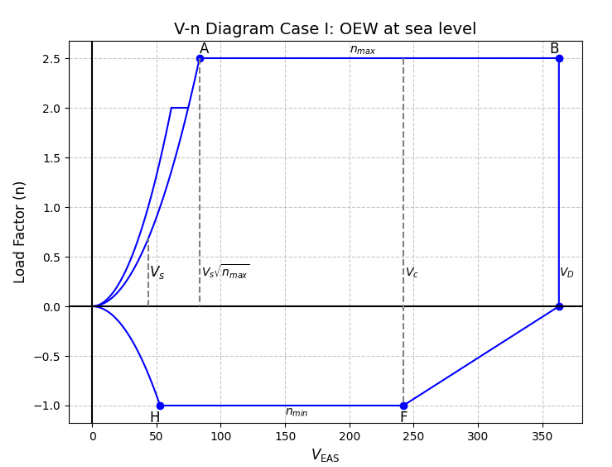
\includegraphics[width=0.65\linewidth]{figures/v-n diagram case I.png}
    \caption{V-n diagram for the aircraft operating at OEW at sea level}
    \label{fig:v-n_case1}
\end{figure}

\begin{figure}[H]
    \centering
    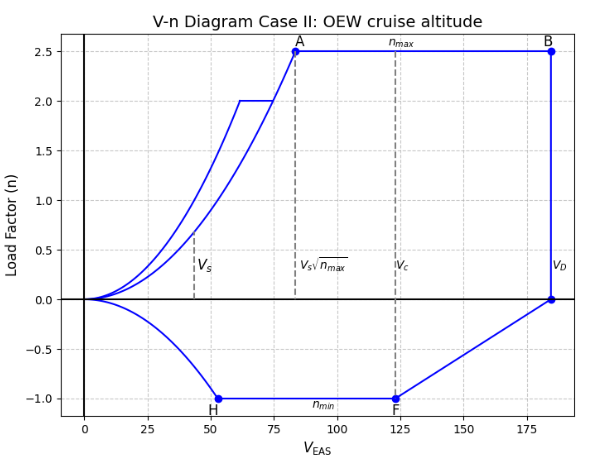
\includegraphics[width=0.65\linewidth]{figures/v-n diagram case II.png}
    \caption{V-n diagram for the aircraft operating at OEW at cruise altitude}
    \label{fig:v-n_case2}
\end{figure}

\begin{figure}[H]
    \centering
    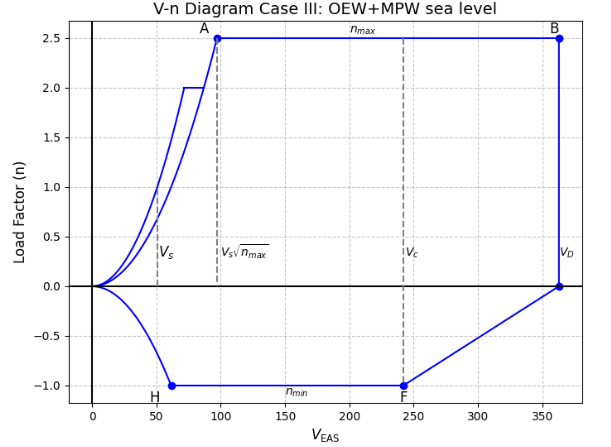
\includegraphics[width=0.65\linewidth]{figures/v-n diagram case III.png}
    \caption{V-n diagram for the aircraft operating at OEW and MPW at sea level}
    \label{fig:v-n_case3}
\end{figure}

\begin{figure}[H]
    \centering
    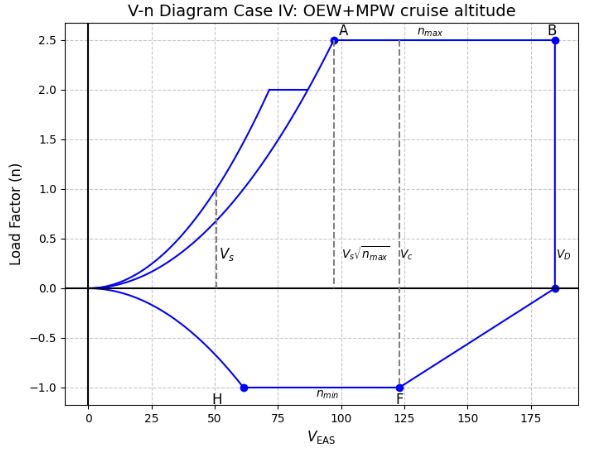
\includegraphics[width=0.65\linewidth]{figures/v-n diagram case IV.png}
    \caption{V-n diagram for the aircraft operating at OEW and MPW at cruise altitude}
    \label{fig:v-n_case4}
\end{figure}

\begin{figure}[H]
    \centering
    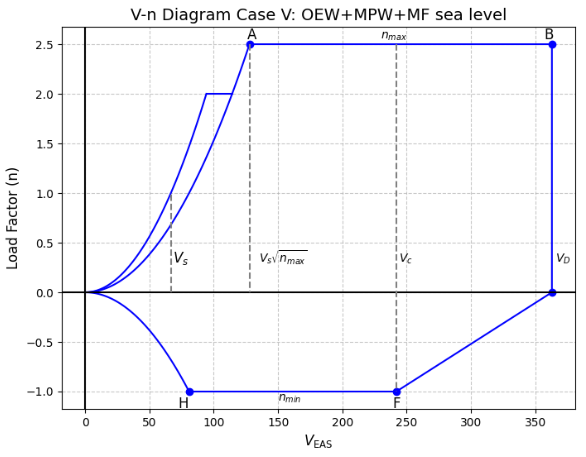
\includegraphics[width=0.65\linewidth]{figures/v-n diagram case V.png}
    \caption{V-n diagram for the aircraft operating at OEW, MPW and MF; at sea level conditions} 
    \label{fig:v-n_case5}
\end{figure}

\begin{figure}[H]
    \centering
    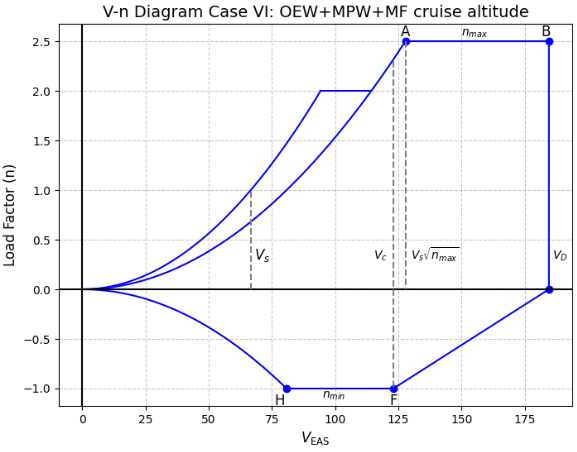
\includegraphics[width=0.65\linewidth]{figures/v-n diagram case VI.png}
    \caption{V-n diagram for the aircraft operating at OEW, MPW and MF; at cruise altitude}
    \label{fig:v-n_case6}
\end{figure}

%% Drag+weight estimation
\end{document}

